\section{Motvating Interoperable Heterogeneous Networks}
Consider the typical hourglass network stack in IP-based networks as shown in left-hand image of Figure \ref{fig:hourglass}. This layered design with a thin-waist infrastructure (IP packets for traffic flow) is what enabled the Internet to grow and expand at such a rapid rate; higher layers in the protocol stack extend this communication medium with support for a variety of applications and networking features (e.g., reliable message traversal via TCP). While the NDN architecture introduces a fundamental paradigm shift in the way information is published and retrieved on a network, its design, shown at a high level in the right-hand image of Figure \ref{fig:hourglass}, borrows the same hourglass design as IP networks. Observe that upper layers of the network stack still promote the development of robust applications based on the underlying communication layers. The difference, however, is that network traffic flow management (i.e., to enable reliable and stable communication) and security are \emph{built into} the network stack. These architectural differences mean that application, transport, and network layer protocol semantics in IP-based networks are distinct from protocol semantics in NDN networks. The NDN gateway is intended to bridge between IP and NDN networks by performing this semantic translation between protocols. 

\begin{figure}[ht!]
\begin{center}
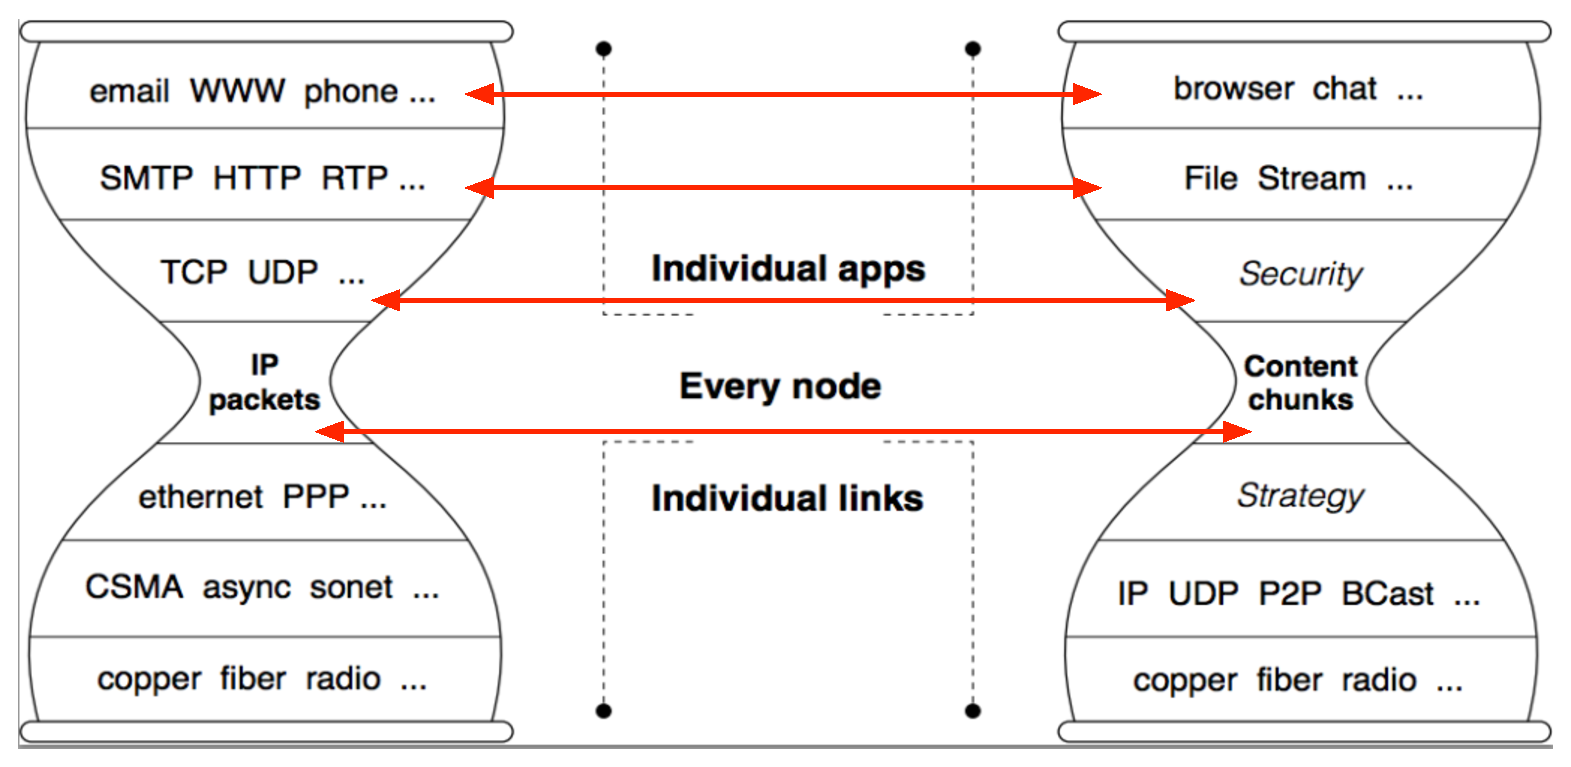
\includegraphics[scale=0.32]{./images/hourglass_conn.pdf}
\label{fig:hourglass}
\caption{A visual comparison of the network stacks for the IP and NDN network architectures.}
\end{center}
\end{figure}

Assuming that NDN is not to be deployed over IP, but instead as a separate network stack entirely, the need for such a gateway cannot be understated. Consider two instances of an application, $A$ and $B$, that wish to send data back and forth to each other. Application $A$ is running on a host with only an IP interface, and application $B$ is running on a host with only an NDN interface. What does it mean for application $A$ to establish a TCP connection stream with application $B$ and what does it mean for application $B$ to issue an interest to application $A$ when neither application speaks the network language of the other. In order for these two applications to communicate, the semantics of a TCP stream-oriented connection must be translated to a stream of contiguous interests, and vice versa. 

Now consider an alternative scenario in which two ``islands'' of NDN hosts exist in isolation, both of which running the same instance of an application. Let host $H_1$ and $H_2$ be a host in the first and second island, respectively, that wish to retrieve data from one another using interests. Without a network route between the two islands, there would be no way for $H_1$ and $H_2$ to interact with one another. However, if there existed two gateways at the borders of each island, each of which connected to the same IP network, then interests from $H_1$ ($H_2$) could be sent to $H_2$ ($H_1)$ as follows:
\begin{enumerate} 
	\item An interest from $H_1$ is intercepted a gateway $G_1$.
	\item $G_1$ encapsulates the interest in an IP packet sent to gateway $G_2$ adhering to IPsec.
	\item $G_2$ unwraps and re-issues the interest and waits for the content to be retrieved from $H_2$. Upon reception, the content's signature is verified and the content is encapsulated in a signed IPsec packet and sent to $G_1$. 
	\item $G_1$ verifies the signature of the packet, creates and signs a new content object, and sends the content object back downstream to $H_1$.
\end{enumerate}

% The gateway middleware is designed so as to support bi-directional traffic flowing from both types of networks. In what follows we describe how traffic in both directions will be supported internally by the gateway.

% \begin{table}[t]
%     \begin{tabular}{|c||c|c|}
%     \hline
%     ~    & {\bf IP} & {\bf NDN} \\ \hline
%     {\bf HTTP} & ~ & ~ \\ \hline
%     {\bf FTP}  & ~ & ~ \\ \hline
%     {\bf SMTP} & ~ & ~ \\ \hline
%     {\bf DNS}  & ~ & ~ \\ \hline
%     \end{tabular}
% \end{table}

\todo[inline]{gateway is two-sided facade}

\section{Network Semantic Translations at the Gateway}
Traditional IP-based applications and upcoming NDN-based applications treat both the network and content in significantly different ways. In IP-based settings, application and transport layer mechanisms and protocols leverage the underlying IP network layer to send packets to specific hosts. In contrast, in NDN-based settings, there are no straightforward application or transport layer analogs; the network layer, responsible for the issuance of interests and retrieval of content, is abstracted to authenticated (i.e., digitally signed) content objects or streams of data that are consumed by applications. From this perspective, there is no clear bijection between application and transport layer communication in IP-based settings and content and stream-centric data retrieval in NDN-settings. Therefore, to support the interoperability of these two networking paradigms, we need a mechanism to translate the semantics of IP-based communication to and from NDN-based content retrieval. 

The direction of traffic across the gateway has a strong influence on how this semantic translation is done: IP-to-NDN application and transport layer protocols will be mapped to corresponding NDN-interests, and NDN-to-IP traffic (in the form of interests) will be encoded so as to map to the appropriate IP-based application or transport layer protocol. Stateless protocols such as HTTP greatly simplify the job of the gateway because it need not maintain any state to support communication across both networks. However, stateful protocols, such as TCP, naturally require the gateway to maintain state so as to emulate the behavior of an endpoint or host that implements such protocols. For instance, if an IP-based application wishes to establish a TCP connection with an application running on an NDN network to retrieve data, then the gateway must maintain stateful information needed to transform streams of data retrieved over a TCP socket to (packed) discrete and contiguous interests in the NDN network. In what follows we describe the semantic translation details for application and transport layer stateful and stateless protocols in both directions across the gateway. 

\begin{figure*}[ht!]
\begin{center}
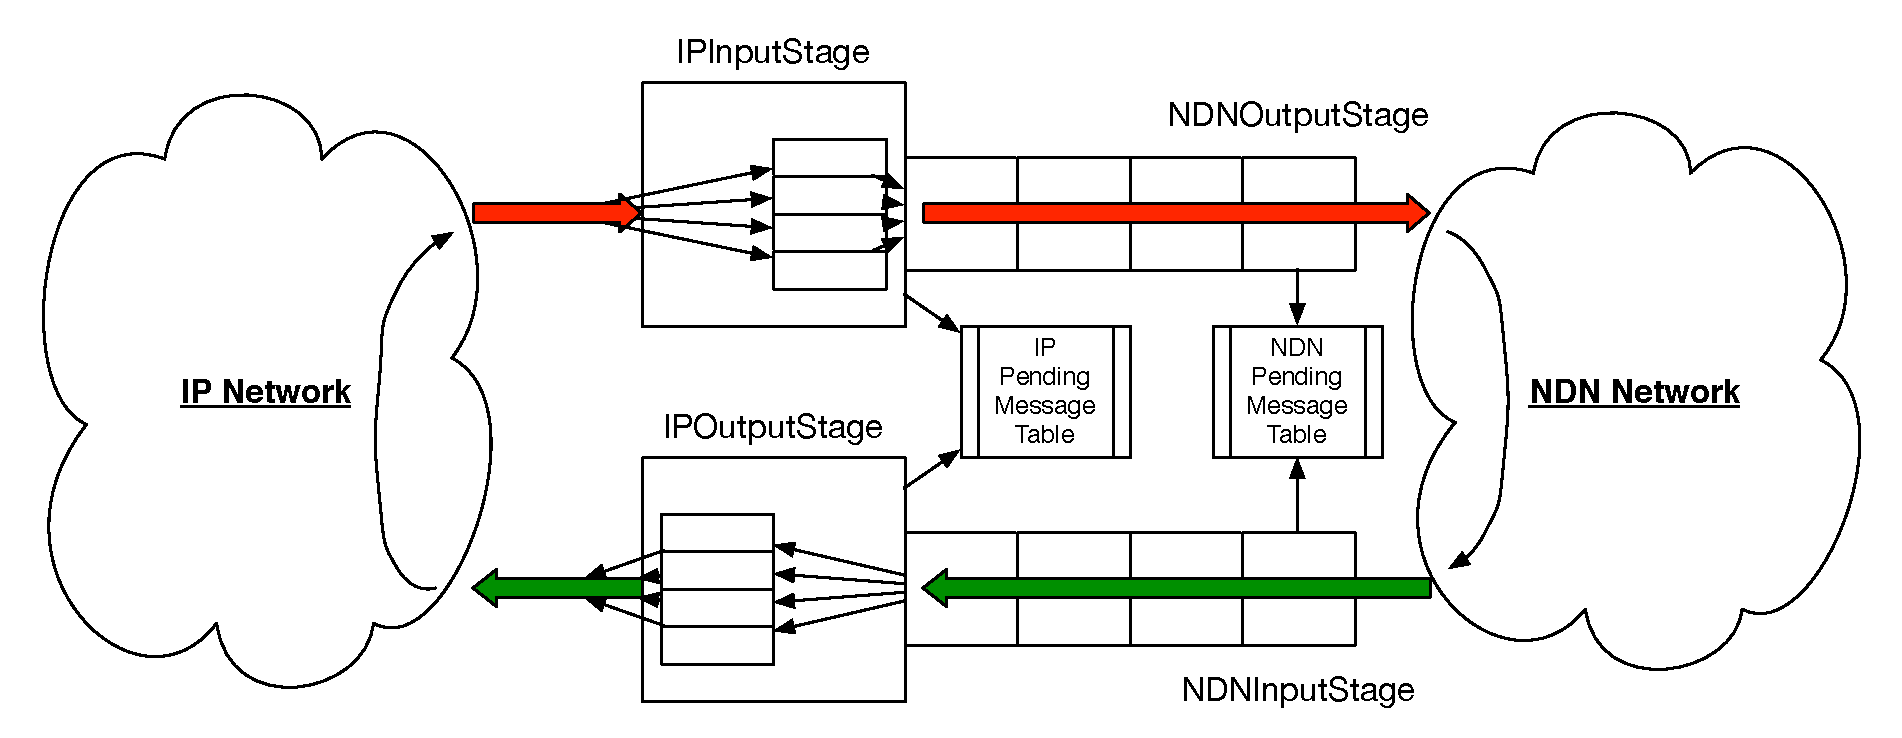
\includegraphics[scale=0.45]{./images/pipeline.pdf}
\label{fig:pipeline}
\caption{Bidirectional message pipeline for IP-to-NDN and NDN-to-IP message traversal.}
\end{center}
\end{figure*}

\subsection{IP-to-NDN Semantic Translation}
TODO

\subsubsection{Application Layer}
Translating IP-based application layer messages to NDN interests is highly dependent on the particular application protocol in question. There is an intuitive NDN-friendly encoding of HTTP GET requests in which human-readable URIs are parsed as interest names. Stateless application-layer protocols enable such direct mappings. Therefore, the gateway supports IP-to-NDN application-layer messaging by encoding interests in HTTP GET requests as follows. NDN content objects with names ``ccnx:/name/of/content'' are issued via the gateway by sending a HTTP GET request with the following format to the gateway (in this example, the IP address X.X.X.X of the gateway is known or can be obtained via DNS):
\begin{center}
GET X.X.X.X:80/ndn/ccnx/name/of/content
\end{center}
Since HTTP requests and NDN interests are stateless, the gateway will parse the URI of the request to determine that (1) it corresponds to an NDN interest, and (2) the full interest name is explicitly ``ccnx:/name/of/content''. Upon reception, the gateway will store the key-value pair $(\mathsf{name}, (\mathsf{source IP}, \mathsf{source port}))$ in the IP pending message table and issue an interest with the given name to the NDN network. Upon receipt of a piece of content, a NDN content handler callback recovers the IP address and port from the pending message table using the content name as the index and then writes the raw content back to the client over the same incoming HTTP TCP connection. Since it is not required that the HTTP request uses a persistent TCP connection, the HTTP message handler is a synchronous procedure that blocks while the NDN interest is satisfied so that the same TCP connection can be used to write the response. 

\subsubsection{Transport Layer}
TODO: interests can be overloaded to contain content, some NDN applications will accept some interests, applications using raw TCP streams to send data to NDN applications, so client opens up TCP socket to gateway and all data is partitioned/packed in an interest/forwarded, setting up TCP connection requires hooking up socket to gateway/sending producer root as first message chunk in TCP stream/and then sending streams of data continually

\subsection{NDN-to-IP Layer Semantic Translation}
Due to their architectural differences, there does not exist a native correspondence between NDN interests and IP-based application layer protocol messages. For example, there is no standard way for a client to represent an HTTP GET request in the format of an NDN interest. To make this type of semantic translation possible, the NDN-to-IP application layer bridge leverages the human-readable names of content to encode IP-based application layer protocol specifics. The encoding for HTTP and FTP semantic translations is specified in EBNF form below; other application-layer protocols can easily be supported by extending this grammar in the natural way.

\todo[inline]{Command pattern}

\begin{figure*}
\begin{mdframed}
\begingrammar
\noindent
<ip-interest>:	'/$\dots$/ip/'<protocol>.

<protocol>:	'http/'<http-cmd>[{'/'<http-path>}] | 'tcp/'<uri-encoded-string>'/'<tcp-ident>. 

<http-cmd>: 'GET' | 'PUT' | 'POST' | 'DELETE'.

% <ftp-cmd>: 'ascii' | 'binary' | 'bye' | 'cd' | 'close' | 'delete' | 'get' | 'help' | 'lcd' | 'ls' | 'mkdir' | 'mget' | 'open' | 'put' | 'pwd' | 'quit' | 'rmdir'.

<http-path>: <uri> | <ip-address>[port]['/'<uri-encoded-string>]

<tcp-ident>: <SHA256-hash>'/'<public-key>.

<tcp-param>: <uri-encoded-string>.

<uri-encoded-string>: TODO

% <number>:	<real-number>;
% 		"$\{$" <real-number> "," <real-number> "$\}$";
% 		{$\backslash$}b[01][01]+;
% 		{$\backslash$}o[07][07]+;
% 		\$[0-9A-Fa-f][0-9A-Fa-f]+.

%<real-number>:	[\+--]?[0-9][0-9]+[\.[0-9]+]?[[eE][0-9][0-9]+].

% <operator>:	"*" |	 "/"	|     "$\backslash$"	| "\%";
% 		"==" |	 "!="	|     "$>$" 		| "$<$"  
% 		| "$<$=" | "$>$=";
% 		"\ul ="	| "\ul !=" |  "\ul $<$" | "\ul $>$" 
% 		| "\ul$<$=" | "\ul$>$=";
% 		"\&"	 | "$\vert$"  | "$\uparrow\uparrow$";
% 		"\&\&"	| "$\Vert$"  | "\ul$\uparrow$".
		
\endgrammar
\end{mdframed}
\end{figure*}

Interests encoded using this grammar are intercepted in the NDNInputStage of the gateway (see Figure \ref{fig:pipeline}). Upon reception, the gateway parses the message, stores a new entry in the NDN pending message table, and forwards the decoded message contents to the appropriate IPOutputStage pipeline stage. Upon reception, the IP response is retrieved in the IPInputStage and forwarded inwards to the NDNOutputStage, where the corresponding entry in the NDN pending message table is indexed using the contents of the arriving message to retrieve the original incoming interest name. Once fetched, the gateway creates and signs a new content object with the IP network response, and then forwards the content downstream to its intended consumer. 

Unlike traditional NDN routing, the gateway pending message table does not collapse interests by default. The reason for this is that application-protocol interests are often issued when \emph{new} state needs to change (i.e., cached responses not generated on demand from the intended IP recipient are not acceptable). 

It is important to note that stateful protocols such as TCP must explicitly embed identifying information about the consumer in order to operate correctly. The reason is that one TCP stream must be associated with at most one consumer, and since NDN does not have any notion of host addresses or identifiers, the consumer application must explicitly encode its identity in the interest. Our grammar enforces identities based on consumer public keys and a corresponding digital signature of the entire interest for such protocols so that consumers can be explicitly identified and their sessions cannot be hijacked by other consumers (doing so would require compromising a consumer and its private key).

\section{Bridging Isolated Networks via Message Encapsulation at the Bridge}
TODO

\section{Internal Gateway Pipeline}
\todo[inline]{pipeline stage defers parsing to subclasses - template pattern}

